\chapter{Classifying Animals}\label{ch:g4:classifying-animals}

A natural history museum keeps millions of \omterm{def:g1:animals-around-us:animal}{animals} --- drawers of
beetles, halls of \omterm{def:g3:bones-and-muscles:skeleton}{skeletons}, jars of \omterm{prop:g3:sorting-living-things:groups}{fish}. Yet a curator can walk
to any one of them in minutes. The secret is not memory but
\emph{order}: every \omterm{def:g1:animals-around-us:animal}{animal} has its place in a great system of
groups within groups, built from the sorting rules of
\cref{ch:g3:sorting-living-things} --- and this year we learn how
the system works.

\section{Groups inside groups}

\begin{definition}[Classification]\label{def:g4:classifying-animals:classification}
To \emph{classify}\index{classify} \omterm{def:g1:living-or-not:living}{living things} is to sort them
by shared body features into groups, and to sort those groups
into bigger groups --- \emph{groups nested inside
groups}\index{nested groups}, like boxes in boxes. The whole
arrangement is a \emph{classification}\index{classification}.
\end{definition}

\begin{example}[The cat's addresses]\label{ex:g4:classifying-animals:cat}
One cat, several nested addresses: the cat is a \emph{mammal}
(\omterm{def:g1:animals-around-us:covering}{fur}, \omterm{def:g2:animals-grow-up:born}{milk} for the young); every mammal is a
\emph{\omterm{def:g4:classifying-animals:vertebrate}{vertebrate}} (a \omterm{def:g3:bones-and-muscles:skeleton}{skeleton} with a \omterm{def:g4:classifying-animals:vertebrate}{backbone} inside); every
\omterm{def:g4:classifying-animals:vertebrate}{vertebrate} is an \emph{\omterm{def:g1:animals-around-us:animal}{animal}}. Cat inside \omterm{prop:g3:sorting-living-things:groups}{mammals}, \omterm{prop:g3:sorting-living-things:groups}{mammals}
inside \omterm{def:g4:classifying-animals:vertebrate}{vertebrates}, \omterm{def:g4:classifying-animals:vertebrate}{vertebrates} inside \omterm{def:g1:animals-around-us:animal}{animals}: each box sits
inside a bigger one.
\end{example}

\begin{definition}[Vertebrates and invertebrates]\label{def:g4:classifying-animals:vertebrate}
A \emph{vertebrate}\index{vertebrate} is an \omterm{def:g1:animals-around-us:animal}{animal} with an inner
\omterm{def:g3:bones-and-muscles:skeleton}{skeleton} built around a \emph{backbone}\index{backbone} --- like
the \omterm{def:g3:bones-and-muscles:skeleton}{spine} you felt in \cref{ex:g3:bones-and-muscles:feel}. An
\omterm{def:g1:animals-around-us:animal}{animal} without a backbone is an
\emph{invertebrate}\index{invertebrate}: \omterm{prop:g3:sorting-living-things:groups}{insects}, spiders,
snails, worms, jellyfish --- the vast majority of all \omterm{def:g1:animals-around-us:animal}{animals}.
\end{definition}

\begin{omfigure}
\begin{tikzpicture}[scale=0.86]
  % outer box: animals
  \draw[thick, omExo] (-0.3,-0.5) rectangle (12.1,4.4);
  \node[font=\small\bfseries, omExo] at (0.9,4.1) {animals};
  % vertebrates box
  \draw[thick, omDef, fill=omDef!4] (0.0,-0.2) rectangle (7.4,3.6);
  \node[font=\small\bfseries, omDef] at (1.35,3.3) {vertebrates};
  \node[font=\footnotesize, omDef] at (2.6,2.85) {(backbone inside)};
  % five classes
  \foreach \x/\name in {0.25/fish, 1.65/amphibians, 3.05/reptiles,
      4.45/birds, 5.85/mammals} {
    \draw[thick, omMeth, fill=omMeth!7] (\x,0.1) rectangle ({\x+1.3},2.4);
    \node[font=\footnotesize, rotate=90] at ({\x+0.65},1.25) {\name};
  }
  % invertebrates box
  \draw[thick, omProp, fill=omProp!5] (7.8,-0.2) rectangle (11.9,3.6);
  \node[font=\small\bfseries, omProp] at (9.2,3.3) {invertebrates};
  \node[font=\footnotesize, align=center] at (9.85,1.4)
    {insects, spiders,\\ snails, worms,\\ jellyfish, \dots\\[3pt]
     (most animals!)};
\end{tikzpicture}

{\small Boxes in boxes: the five classes of \omterm{def:g4:classifying-animals:vertebrate}{vertebrates} together
form one box, sitting beside the far more crowded \omterm{def:g4:classifying-animals:vertebrate}{invertebrates},
inside the box of all \omterm{def:g1:animals-around-us:animal}{animals}.}
\end{omfigure}

\section{The five classes of vertebrates}

\begin{proposition}[The five vertebrate classes]\label{prop:g4:classifying-animals:classes}
\omterm{def:g4:classifying-animals:vertebrate}{Vertebrates} are classified into five great groups, called
\emph{classes}\index{class (of vertebrates)}:
\begin{enumerate}
  \item \emph{\omterm{prop:g3:sorting-living-things:groups}{fish}}: scales, fins, breathe in water --- trout,
        shark, sardine;
  \item \emph{amphibians}\index{amphibian}: moist bare \omterm{def:g1:the-five-senses:sense}{skin},
        \omterm{def:g2:animals-grow-up:born}{eggs} in water, tadpole childhood --- frog, toad, newt;
  \item \emph{reptiles}\index{reptile}: dry scaly \omterm{def:g1:the-five-senses:sense}{skin}, most lay
        shelled \omterm{def:g2:animals-grow-up:born}{eggs} on land --- lizard, snake, tortoise,
        crocodile;
  \item \emph{\omterm{prop:g3:sorting-living-things:groups}{birds}}: \omterm{def:g1:animals-around-us:covering}{feathers}, beak, shelled \omterm{def:g2:animals-grow-up:born}{eggs} --- blackbird,
        ostrich, penguin;
  \item \emph{\omterm{prop:g3:sorting-living-things:groups}{mammals}}: \omterm{def:g1:animals-around-us:covering}{fur} or hair, young fed on \omterm{def:g2:animals-grow-up:born}{milk} --- cat,
        whale, bat, human.
\end{enumerate}
\end{proposition}
\admitted

\begin{example}[Sorting a zoo delivery]\label{ex:g4:classifying-animals:zoo}
Six crates arrive: a python (dry scaly \omterm{def:g1:the-five-senses:sense}{skin}, shelled \omterm{def:g2:animals-grow-up:born}{eggs} ---
reptile), a toad (moist bare \omterm{def:g1:the-five-senses:sense}{skin} --- amphibian), a penguin
(\omterm{def:g1:animals-around-us:covering}{feathers} --- bird), a shark (fins and gills --- \omterm{prop:g3:sorting-living-things:groups}{fish}), a
dolphin (\omterm{def:g2:animals-grow-up:born}{milk} for its calf --- mammal), and a crate of giant
snails (no \omterm{def:g4:classifying-animals:vertebrate}{backbone} at all --- \omterm{def:g4:classifying-animals:vertebrate}{invertebrates}, in no \omterm{def:g4:classifying-animals:vertebrate}{vertebrate}
class whatever).
\end{example}

\begin{remark}[Reptile or amphibian?]\label{rem:g4:classifying-animals:confusion}
Lizards and newts look alike at a glance --- four \omterm{def:g1:my-body:parts}{legs}, long
tail. The \omterm{def:g1:the-five-senses:sense}{skin} decides: the lizard's is dry and scaly, the
newt's moist and bare; the lizard's \omterm{def:g2:animals-grow-up:born}{eggs} have \omterm{def:g1:animals-around-us:covering}{shells} and are
laid on land, the newt's are laid bare in water. Same
silhouette, different classes.
\end{remark}

\section{Using a classification}

\begin{method}[Placing a vertebrate in its class]\label{met:g4:classifying-animals:place}
Ask the questions in order, stopping at the first yes:
\begin{enumerate}
  \item \omterm{def:g1:animals-around-us:covering}{Feathers}? --- a bird.
  \item \omterm{def:g1:animals-around-us:covering}{Fur} or hair (or \omterm{def:g2:animals-grow-up:born}{milk} for the young)? --- a mammal.
  \item Dry scaly \omterm{def:g1:the-five-senses:sense}{skin}? --- a reptile.
  \item Moist bare \omterm{def:g1:the-five-senses:sense}{skin} and a tadpole childhood? --- an
        amphibian.
  \item Fins and gills, life in water? --- a \omterm{prop:g3:sorting-living-things:groups}{fish}.
\end{enumerate}
No \omterm{def:g4:classifying-animals:vertebrate}{backbone} at all? Then it was an \omterm{def:g4:classifying-animals:vertebrate}{invertebrate}, and the
questions do not apply.
\end{method}

\begin{proposition}[What a class tells you for free]\label{prop:g4:classifying-animals:free}
Knowing an \omterm{def:g1:animals-around-us:animal}{animal}'s class is knowing a bundle of facts before
looking: told only ``it is a mammal'', you already expect \omterm{def:g1:animals-around-us:covering}{fur}, \omterm{def:g2:animals-grow-up:born}{milk}
for the young, and --- like nearly all \omterm{prop:g3:sorting-living-things:groups}{mammals} --- young \omterm{def:g2:animals-grow-up:born}{born
alive}. That saving is the whole point of \omterm{def:g4:classifying-animals:classification}{classification}: learn
the group once, and every member arrives half-known.
\end{proposition}
\admitted

\begin{example}[A new species arrives]\label{ex:g4:classifying-animals:new}
Naturalists still discover \omterm{def:g1:animals-around-us:animal}{animals} never seen before. When a new
bat-like \omterm{def:g1:animals-around-us:animal}{animal} is found with \omterm{def:g1:animals-around-us:covering}{fur} and \omterm{def:g2:animals-grow-up:born}{milk}, it goes straight
into the \omterm{prop:g3:sorting-living-things:groups}{mammals} --- and at once biologists expect a \omterm{def:g4:classifying-animals:vertebrate}{backbone}, a
four-chambered heart and warm blood, before any of it is
checked. The \omterm{def:g4:classifying-animals:classification}{classification} pays out predictions.
\end{example}

\begin{remark}[Toward the family tree]\label{rem:g4:classifying-animals:tree}
Why do \omterm{def:g1:animals-around-us:covering}{fur}, \omterm{def:g2:animals-grow-up:born}{milk} and \omterm{def:g4:classifying-animals:vertebrate}{backbones} travel together so faithfully?
The full answer --- that members of a group inherit their shared
features from common ancestors --- belongs to the story of
kinship and evolution, taken up in later years. For now, the
nested boxes simply work, and work marvellously.
\end{remark}

\begin{omfigure}
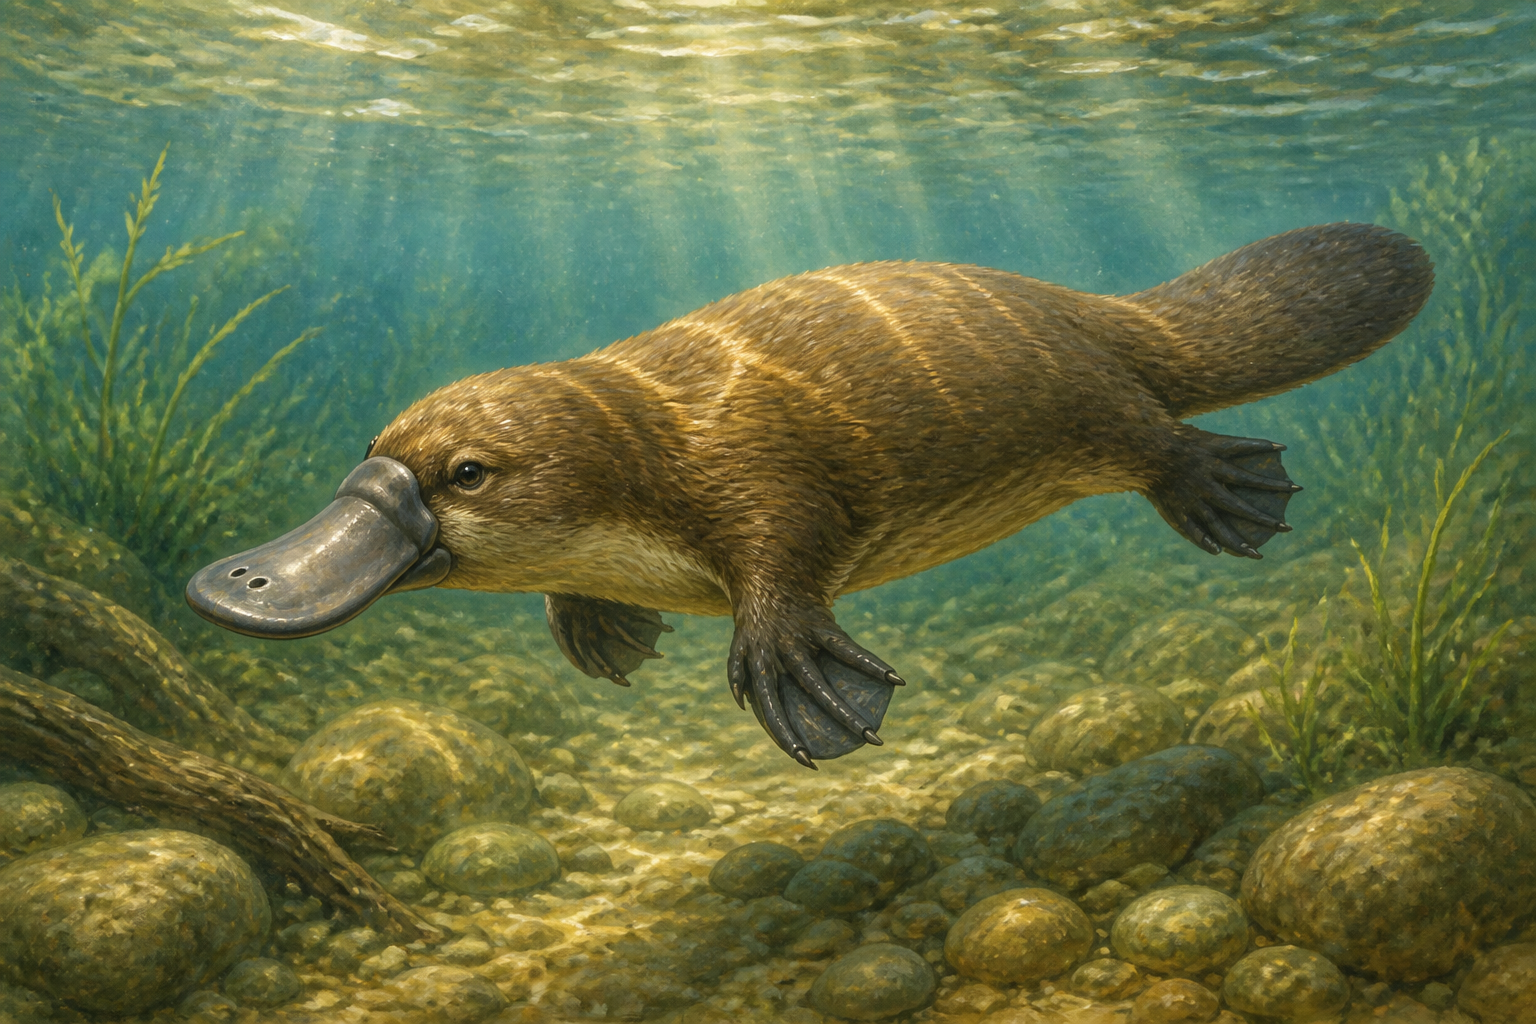
\includegraphics[width=0.6\linewidth]{images/book1/ai/g4-classify-platypus.png}

{\small The classifier's favorite headache: \omterm{def:g1:animals-around-us:covering}{fur} and \omterm{def:g2:animals-grow-up:born}{milk}, but a
bill, webbed feet --- and \omterm{def:g2:animals-grow-up:born}{eggs}. The platypus (see the last
exercise) tests the whole method.}
\end{omfigure}

\section{Exercises}

\begin{exercise}[$\star$]\label{exo:g4:classifying-animals:1}
What is a \omterm{def:g4:classifying-animals:vertebrate}{vertebrate}? What is an \omterm{def:g4:classifying-animals:vertebrate}{invertebrate}? Give two examples
of each.
\end{exercise}

\begin{exercise}[$\star$]\label{exo:g4:classifying-animals:2}
Name the five classes of \omterm{def:g4:classifying-animals:vertebrate}{vertebrates} with their defining
features.
\end{exercise}

\begin{exercise}[$\star$]\label{exo:g4:classifying-animals:3}
Place each \omterm{def:g1:animals-around-us:animal}{animal}: the sardine, the crocodile, the newt, the
ostrich, the whale, the earthworm.
\end{exercise}

\begin{exercise}[$\star$]\label{exo:g4:classifying-animals:4}
Write the cat's nested addresses, smallest box to biggest, as in
\cref{ex:g4:classifying-animals:cat}.
\end{exercise}

\begin{exercise}[$\star$]\label{exo:g4:classifying-animals:5}
A lizard and a newt look alike. Which two features separate
their classes?
\end{exercise}

\begin{exercise}[$\star$]\label{exo:g4:classifying-animals:6}
Which group holds the vast majority of all \omterm{def:g1:animals-around-us:animal}{animals}? Name four of
its members.
\end{exercise}

\begin{exercise}[$\star$]\label{exo:g4:classifying-animals:7}
Run \cref{met:g4:classifying-animals:place} aloud on the
penguin and on the dolphin, question by question.
\end{exercise}

\begin{exercise}[$\star$]\label{exo:g4:classifying-animals:8}
You are told only: ``this \omterm{def:g1:animals-around-us:animal}{animal} is a bird.'' List three things
you now expect without looking, by
\cref{prop:g4:classifying-animals:free}.
\end{exercise}

\begin{exercise}[$\star\star$]\label{exo:g4:classifying-animals:9}
The whale has almost no hair and lives like a \omterm{prop:g3:sorting-living-things:groups}{fish}. Using
\cref{met:g4:classifying-animals:place} and
\cref{ex:g3:sorting-living-things:surprises}, explain why it is
nonetheless a mammal --- and why ``lives in the sea'' never
was a \omterm{def:g4:classifying-animals:classification}{classification} feature.
\end{exercise}

\begin{exercise}[$\star\star$]\label{exo:g4:classifying-animals:10}
The snake has no \omterm{def:g1:my-body:parts}{legs}, and neither has the earthworm. Why is
one a \omterm{def:g4:classifying-animals:vertebrate}{vertebrate} reptile and the other an \omterm{def:g4:classifying-animals:vertebrate}{invertebrate}? Which
single feature outranks the missing \omterm{def:g1:my-body:parts}{legs}?
\end{exercise}

\begin{exercise}[$\star\star\star$]\label{exo:g4:classifying-animals:11}
The platypus puzzled naturalists: \omterm{def:g1:animals-around-us:covering}{fur} and \omterm{def:g2:animals-grow-up:born}{milk}, yet it lays
shelled \omterm{def:g2:animals-grow-up:born}{eggs}. Which class won, and why? What does the puzzle
show about classifying by \emph{bundles} of features rather
than by a single one?
\end{exercise}
